\section{Chernoff's Bound}

% [CORRECTED] was: the paragraph left $p$ free --- the expected degree of a vertex of $G_{n, p}$ is $(n-1)p$, and
% every number in this discussion (the interval $(0.49n, 0.51n)$, the $\delta = 0.01$, the variance below) is the
% one belonging to $p = \frac{1}{2}$.
Consider a random graph $G_{n, p}$ with $n$ vertices and edges chosen uniformly at random with probability $p$, and take $p = \frac{1}{2}$ for this discussion.

The expected degree of a vertex is $\frac{n-1}{2}$.

How many vertices have degrees lying in $(0.49n, 0.51n)$? We can actually show that
% [CORRECTED] was: "$\to 1$" at the end of the display --- $n$ is bound by the limit, so there is no index left for
% an arrow to run along; what the display asserts is that the limit exists and equals $1$.
\begin{align*}
    \lim_{n \to \infty} \Pr\of{\text{every vertex in $G_{n, p}$ has degree in $(0.49n, 0.51n)$}} = 1
\end{align*}
% [CORRECTED] was: "$\Var{\deg(x)} = \frac{n-1}{2}$" --- that is the expectation written twice. A sum of $n - 1$
% independent Bernoulli$\parenth{\frac{1}{2}}$ variables has variance $\frac{n-1}{4}$, which is what the Chebyshev
% display below already uses.
Indeed, fix a vertex $x$. $\deg(x)$ is a binomial random variable, counting the $n - 1$ possible edges at $x$, each present independently. $\E\of{\deg(x)} = \frac{n-1}{2}$ and $\Var{\deg(x)} = \frac{n-1}{4}$.

% [CORRECTED] was: "$\approx \frac{1}{\delta^2 n}$", and "$\frac{10,000}{n}$" after it --- $\frac{(n-1)/4}{\delta^2 n^2}$ is
% asymptotically $\frac{1}{4 \delta^2 n}$, and the coin-flipping example above does the same computation keeping the
% factor of $4$. The point of the passage, that the bound is useless, survives either number.
Applying Chebyshev gives us
\begin{align*}
    \Pr\of{\abs{\deg(x) - \frac{n-1}{2}} \geq \delta n} \leq \frac{\frac{n-1}{4}}{(\delta n)^2}
    \approx \frac{1}{4 \delta^2 n}
\end{align*}
But this is a rather terrible bound: for $\delta = 0.01$, this is already $\frac{2,500}{n}$. Saying a probability is less than or equal to this is essentially useless!

We can consider taking higher moment bounds: bounding using not the second power of $X - \E(X)$, but the fourth or sixth or eighth power. In this instance, a fourth power bound would actually be enough. But that won't always be the case.

What's one thing that beats \textit{all} of these? An exponential!

% [CORRECTED] was: "$\eta := \sum_{i=1}^{n} \xi_n$" --- the summand does not depend on the index, so that sum is
% $n \xi_n$, a single scaled coin flip of variance $n^2$; the theorem below, and its factorization over $i$, need
% the walk $\sum_i \xi_i$.
% [SUSPECT] "the binomial random variable $\eta$" below: $\eta = 2B - n$ for $B$ binomial, so its support is
% $\set{-n, -n+2, \ldots, n}$ and it is not binomial. Two independent reviewers called this wrong and I left it,
% on the grounds that naming a variable after the distribution it is an affine image of is loose rather than
% false --- and because $\deg(x)$ two pages earlier is binomial in the literal sense, so the word is doing two
% jobs. One word, and it is the author's to change.
Consider the following setup. Let $\xi_1, \ldots, \xi_n$ be independent Bernoulli random variables take values $\pm 1$ with probability $\frac{1}{2}$. Define the binomial random variable $\eta := \sum_{i=1}^{n} \xi_i$.

% [CORRECTED] was: "$\Pr\of{\eta > a} = \Pr\of{\beta^2 > \beta^a} \leq \E\of{\beta^2}$" --- $\beta^2$ is a constant, so
% the middle probability is $0$ or $1$ and says nothing about $\eta$; and Markov's inequality divides by the
% threshold, which had been dropped.
Note that because $x < y \iff e^x < e^y$, we get that
\begin{align*}
    \Pr\of{\eta \geq a} = \Pr\of{\beta^{\eta} \geq \beta^a} \leq \frac{\E\of{\beta^{\eta}}}{\beta^a}
\end{align*}
by Markov's inequality (where $\beta$ denotes $e^t$ for $t > 0$, a bit like how $q$ denotes $e^{2 \pi i z}$).

Optimizing over $t$ turns that into a bound that decays in $a$ faster than any power.

\begin{boxtheorem}[Chernoff's Bound] \label{Ch4:Thm:Chernoff}
    Let $\xi_1, \ldots, \xi_n$ be independent random variables each taking the values $\pm 1$ with probability $\frac{1}{2}$, and let $\eta = \sum_{i=1}^{n} \xi_i$. Then for every $a \geq 0$,
    \begin{align*}
        \Pr\of{\eta \geq a} \leq e^{-\frac{a^2}{2n}}
    \end{align*}
\end{boxtheorem}
\begin{proof}
    At $a = 0$ the bound reads $\Pr\of{\eta \geq 0} \leq 1$ and there is nothing to prove, so take $a > 0$, and fix $t > 0$ for the moment. Notice that
    \begin{align*}
        \E\of{e^{t \eta}}
        = \E\of{e^{t \sum_{i=1}^{n} \xi_i}}
        = \E\of{\prod_{i=1}^{n} e^{t \xi_i}}
        = \prod_{i=1}^{n} \E\of{e^{t \xi_i}}
        = \parenth{\frac{e^{-t} + e^{t}}{2}}^{n}
    \end{align*}
    % Not from the lecture: the lecture asserted the bound on the display below; the comparison of the two series was supplied.
    % [CORRECTED] was: an equality at the end of the display below --- $\E\of{e^{t\eta}} = \parenth{\cosh t}^n$ is
    % strictly less than $e^{t^2 n / 2}$ for every $t \neq 0$, and the step is the inequality just established.
    the third equality by independence. Comparing the series termwise, $\frac{e^{t} + e^{-t}}{2} = \sum_{k \geq 0} \frac{t^{2k}}{(2k)!} \leq \sum_{k \geq 0} \frac{t^{2k}}{2^k k!} = e^{\frac{t^2}{2}}$, since $(2k)! \geq 2^k k!$. We therefore conclude that
    \begin{align*}
        \Pr\of{\eta \geq a}
        = \Pr\of{e^{t\eta} \geq e^{ta}}
        \leq \frac{\E\of{e^{t \eta}}}{e^{ta}}
        \leq e^{\frac{t^2 n}{2} - ta}
    \end{align*}
    % [CORRECTED] was: "the $n$ that minimises this" --- $n$ is fixed by the statement and the exponent is increasing
    % in it; the free parameter is $t$, and $t = \frac{a}{n}$ is what gives $e^{-a^2 / 2n}$.
    Can we optimize this? Ie, can we find the $t$ that minimizes this? It turns out, we can: by some calculus nonsense, we get that the optimal value is $e^{-\frac{a^2}{2n}}$.
\end{proof}

The same bound holds if the $\xi_i$ are independent and for all $i$, $\abs{\xi_i} \leq 1$ and $\E\of{\xi_i} = 0$.

% [CORRECTED] was: "let $\eta$ denote their product" --- the display immediately below factorizes $\E\of{e^{t\eta}}$
% over $i$, which is the exponential turning a sum into a product, and a bound of the shape $e^{-a^2/2n}$ only has
% content for a sum.
For instance, consider the case where
\begin{align*}
    \xi_i =
    \begin{cases}
        \frac{1}{3} & \text{ with probability } \frac{3}{4} \\
        -1 & \text{ with probability } \frac{1}{4}
    \end{cases}
\end{align*}
and as before, let $\eta$ denote their sum. By the same sort of technology we used above,
\begin{align*}
    \E\of{e^{t \eta}} = \prod_{i=1}^{n} \E\of{e^{t\xi_i}}
\end{align*}
Define
\begin{align*}
    h(x) = \frac{e^{t} + e^{-t}}{2} + x \frac{e^{t} - e^{-t}}{2}
\end{align*}
We can show that
\begin{align*}
    \E\of{e^{t \xi_i}}
    \leq \E\of{h\of{\xi_i}}
    = h\of{\E\of{\xi_i}}
    = h(0)
    = \frac{e^t + e^{-t}}{2}
\end{align*}
The first inequality is the whole content of the extension: $h$ is the chord of $x \mapsto e^{tx}$ across $[-1, 1]$, and since $e^{tx}$ is convex it lies below that chord on the whole interval, which is where $\abs{\xi_i} \leq 1$ is used. The first equality is linearity, since $h$ is affine, and the second is where $\E\of{\xi_i} = 0$ is used.

\begin{figure}[H]
    \centering
    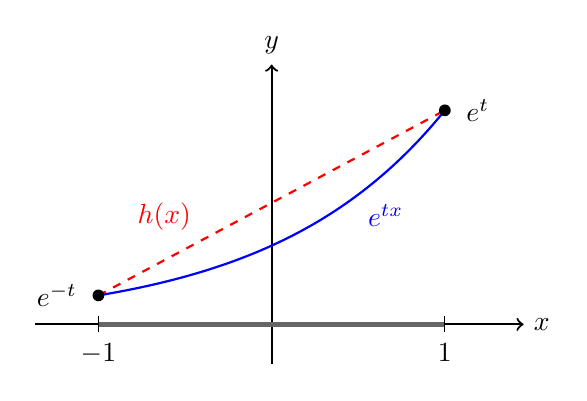
\begin{tikzpicture}
        \draw[thick, ->] (-3, 0) -- (3.2, 0) node[anchor = west] {$x$};
        \draw[thick, ->] (0, -0.5) -- (0, 3.3) node[anchor = south] {$y$};
        \draw[line width = 1.6pt, black!60] (-2.2, 0) -- (2.2, 0);
        \draw (-2.2, -0.1) -- (-2.2, 0.1);
        \draw (2.2, -0.1) -- (2.2, 0.1);
        \node[anchor = north] at (-2.2, -0.12) {$-1$};
        \node[anchor = north] at (2.2, -0.12) {$1$};
        \draw[thick, blue, domain = -1:1, samples = 80] plot ({2.2 * \x}, {exp(\x)});
        \node[anchor = north west, blue] at (1.1, 1.65) {$e^{tx}$};
        \draw[thick, dashed, red] (-2.2, 0.3679) -- (2.2, 2.7183);
        \node[anchor = south east, red] at (-0.9, 1.0632) {$h(x)$};
        \node[circle, fill = black, inner sep = 1.5pt] at (-2.2, 0.3679) {};
        \node[circle, fill = black, inner sep = 1.5pt] at (2.2, 2.7183) {};
        \node[anchor = east] at (-2.35, 0.3679) {$e^{-t}$};
        \node[anchor = west] at (2.35, 2.7183) {$e^{t}$};
    \end{tikzpicture}
\end{figure}
